\chapter{The NED Language}
\label{cha:the-ned-language}


\section{NED overview}

The user describes the structure of a simulation model in the NED language. NED
stands for Network Description. NED lets the user declare simple modules, and
connect and assemble them into compound modules. The user can label some compound
modules as \textit{networks}, self-contained simulation models. Channels are
another component type, whose instances can also be used in compound modules.

The NED language has several features which let it scale well to large projects:

\begin{description}

\item[Hierarchical] The traditional way to deal with complexity is via
introducing hierarchies. In {\opp}, any module which would be too complex as
a single entity can be broken down into smaller modules, and used as a
compound module.

\item[Component-Based] Simple modules and compound modules are inherently
reusable, which not only reduces code copying, but more importantly, allows
component libraries (like the INET Framework, MiXiM, Castalia, etc.) to
exist.

\item[Interfaces] Module and channel interfaces can be used as a
placeholder where normally a module or channel type would be used, and the
concrete module or channel type is determined at network setup time by a
parameter. Concrete module types have to ``implement'' the interface they
can substitute. For example, given a compound module type named
\ttt{MobileHost} contains a \ttt{mobility} submodule of the type
\ttt{IMobility} (where \ttt{IMobility} is a module interface), the actual
type of \ttt{mobility} may be chosen from the module types that implemented
\ttt{IMobility} (\ttt{RandomWalkMobility}, \ttt{TurtleMobility}, etc.)

\item[Inheritance] Modules and channels can be subclassed. Derived modules
and channels may add new parameters, gates, and (in the case of compound
modules) new submodules and connections. They may set existing parameters
to a specific value, and also set the gate size of a gate vector. This
makes it possible, for example, to take a \ttt{GenericTCPClientApp} module
and derive an \ttt{FTPClientApp} from it by setting certain parameters to a fixed
value; or to derive a \ttt{WebClientHost} compound module from a
\ttt{BaseHost} compound module by adding a \ttt{WebClientApp} submodule and
connecting it to the inherited \ttt{TCP} submodule.

\item[Packages] The NED language features a Java-like package structure,
to reduce the risk of name clashes between different models. \ttt{NEDPATH}
(similar to Java's \ttt{CLASSPATH}) was also introduced to make it easier
to specify dependencies among simulation models.

\item[Inner types] Channel types and module types used locally by a
compound module can be defined within the compound module, in order to
reduce namespace pollution.

\item[Metadata annotations] It is possible to annotate module or channel
types, parameters, gates and submodules by adding properties. Metadata are
not used by the simulation kernel directly, but they can carry extra
information for various tools, the runtime environment, or even for other
modules in the model. For example, a module's graphical representation
(icon, etc)  or the prompt string and measurement unit (milliwatt, etc) of a
parameter are already specified as metadata annotations.

\end{description}

\begin{note}
    The NED language has changed significantly in the 4.0 version.
    Inheritance, interfaces, packages, inner types, metadata annotations, inout
    gates were all added in the 4.0 release, together with many other features.
    Since the basic syntax has changed as well, old NED files need to be
    converted to the new syntax. There are automated tools for this purpose, so
    manual editing is only needed to take advantage of new NED features.
\end{note}

The NED language has an equivalent tree representation which can be
serialized to XML; that is, NED files can be converted to XML and back
without loss of data, including comments. This lowers the barrier for
programmatic manipulation of NED files, for example extracting information,
refactoring and transforming NED, generating NED from information stored in
other system like SQL databases, and so on.

\begin{note}
    This chapter is going to explain the NED language gradually, via examples.
    If you are looking for a more formal and concise treatment, see
    Appendix \ref{cha:ned-language-grammar}.
\end{note}


\section{Simple modules, compound modules, networks}

In this section we introduce the NED language via a complete and
reasonably real-life example: a communication network.

Our hypothetical network consists of nodes. One each node there's an
application running which generates packets at random intervals.
The nodes are routers themselves as well, and the network is connected
by 1 megabit/sec lines. We assume that the application uses datagram-based
communication, so that we can leave out the transport layer from the model.

Our simulation model will look like this:

TODO screenshot of one node
TODO screenshot of the network

Let us build the model bottom-up. First we define the simple module
types that will make up a network node. We need an application;
a module that performs network layer functions including routing;
and a module that queues up packets before they are transmitted on the
line. A NED file that declares them would look like this:

\begin{Verbatim}[commandchars=\\\{\}]
simple App
\{
    parameters:
        int address;  // local node address
        string destAddresses;  // destination addresses
        volatile double sendIaTime @unit(s) = default(exponential(1s));
                               // time between generating packets
        volatile int packetLength @unit(byte);  // length of one packet
        @display("i=block/browser");
    gates:
        input in;
        output out;
\}

simple Routing
\{
    parameters:
        @display("i=block/switch");
    gates:
        input in[];
        output out[];
        input localIn;
        output localOut;
\}

simple L2Queue
\{
    parameters:
        int frameCapacity = default(0); // max queue length; 0 means no limit
        @display("i=block/queue;q=queue");
    gates:
        input in;
        output out;
        inout line;
\}
\end{Verbatim}

It would also be possible (moreover, recommended) to put the above three
simple module declarations into separate \ttt{.ned} files: \ttt{App.ned},
\ttt{Routing.ned} and \ttt{L2Queue.ned}. Note that the NED language uses
the familiar curly brace syntax, and ``\ttt{//}'' to denote comments.

Let us see the first simple module type declaration. It declares a
\textit{module type} named \ttt{App}, which has four \textit{parameters}
called \ttt{address}, \ttt{destAddresses}, \ttt{sendIaTime} and \ttt{packetLength},
and also two \textit{gates} named \ttt{in} and \ttt{out}. The argument of
\ttt{@display()} is called a \textit{display string}, and it defines
the default rendering of the module in graphical environments;
\ttt{"i=..."} defines the default icon.

\begin{note}
    Note that the module type names (\ttt{App}, \ttt{Routing}, \ttt{L2Queue})
    begin with a capital letter, and parameter and gate names begin with
    lowercase -- this is the recommended naming convention. Capitalization
    matters because the language is case sensitive.
\end{note}

Notice that the declarations don't contain any code to define the operation
of the application (routing algorithm, queue) itself:
that part is expressed in C++. By default, {\opp} looks for a
C++ class of the same name (so here, \ttt{App}, \ttt{Routing} and {L2Queue}),
although this gets slightly more complicated if C++ namespaces or
NED packages are involved, and the user can also explicitly specify
which C++ class to use.

\ttt{App}'s parameters are of various data types (\ttt{int}, \ttt{double},
\ttt{string}) and some of them are also declared \ttt{volatile}. Parameters
can be read into C++ variables of similar types, and can be used by the
algorithm that drives the simple module. \ttt{volatile} practically means
that the parameter can be used as a source of random numbers.

\begin{note}
    With constructs like \ttt{exponential(1s)} assigned to the \ttt{sendIaTime}
    parameter in this example, \ttt{volatile} effectively means that
    there is no need to ever hardcode the distribution (e.g. "normal")
    into the C++ code, or to use multiple parameters to pass its mean,
    standard deviation etc into the C++ code. A single parameter can
    encapsulate all details, and can provide any random variable.
\end{note}

The \ttt{@unit(s)} and \ttt{@unit(byte)} bits declare the measurement unit
for the parameter. Values assigned to parameters must have the same or
compatible unit, i.e. \ttt{@unit(s)} accepts milliseconds, nanoseconds,
minutes, hours, etc., and \ttt{@unit(byte)} accepts kilobytes, megabytes,
etc. as well.

Generally, \ttt{@}-words like \ttt{@unit} and \ttt{@display} are called
\textit{properties} in NED, and they are used to annotate various objects
with metadata. Properties can be attached to parameters, gates, modules,
connections and other objects.

Both the \ttt{parameters:} and \ttt{gates:} sections in the simple module are
optional, that is, they can be left out if there's no parameter or gate.

Simple modules can be extended (or specialized) via subclassing. This will be
discussed in section \ref{sec:ch-ned-lang:inheritance}.

Comments in the NED source also serve a purpose in addition to making
the NED source more readable: in the {\opp} IDE they get displayed
at various places (tooltips, content assist, etc), and become part
of the documentation extracted from the NED files.
The NED documentation system, not unlike \textit{JavaDoc}
or \textit{Doxygen}, will be described in Chapter \ref{cha:neddoc}.

Now that we've learned enough about simple modules, we assemble our components
into a compound module type that represents a network node:

\begin{Verbatim}[commandchars=\\\{\}]
module Node
\{
    parameters:
        int address;
        @display("i=misc/node_vs,gold");
    gates:
        inout port[];
    submodules:
        app: App \{
            parameters:
                address = address;
                @display("p=140,60");
        \}
        routing: Routing \{
            parameters:
                @display("p=140,130");
            gates:
                in[sizeof(port)];
                out[sizeof(port)];
        \}
        queue[sizeof(port)]: L2Queue \{
            parameters:
                @display("p=80,200,row");
        \}
    connections:
        routing.localOut --> app.in;
        routing.localIn <-- app.out;
        for i=0..sizeof(port)-1 \{
            routing.out[i] --> queue[i].in;
            routing.in[i] <-- queue[i].out;
            queue[i].line <--> port[i];
        \}
\}
\end{Verbatim}

A compound module type, like simple modules, may have parameters and gates.
Our \ttt{Node} module contains an \ttt{address} parameter, plus a
\textit{gate vector} of unspecified size, named \ttt{port}.
The actual gate vector size will be determined implicitly by the number
of neighbours when we create a network from nodes of this type.
The type of \ttt{port[]} is \ttt{inout}, which basically means that
each gate is in fact a pair of gates, an input and an output gate;
they can also be addressed individually if needed, as \ttt{port\$i} and
\ttt{port\$o} (or rather, \ttt{port\$i[$k$]} and \ttt{port\$o[$k$]},
because now we have a gate vector.) Gate vectors can also be created with
a specified size, or be set to a fixed size at the place
of instantiating the module.

The point of compound modules is to serve as a container for other
modules. Our \ttt{Node} compound module type has an \ttt{app} and
a \ttt{routing} \textit{submodule}, plus a \ttt{queue[]} \textit{submodule vector}
that contains one \ttt{L2Queue} module for each port, as specified by
\ttt{[sizeof(port)]}.
Any module type (simple or compound module) can be used as a submodule.
Like simple modules, compound modules can also have gates and parameters,
and they can be used wherever simple modules can be used.

It is useful to think about compound modules as ``cardboard boxes''
that help you organize your simulation model and bring structure into
it. No active behaviour is associated with compound modules -- they
are simply meant for grouping modules into larger units that can
can be used either as a model (a \textit{network}, see later)
or as a building block for other compound modules.

Syntactically, a submodule may have a curly brace block as body, where
it is possible to assign its parameters (see \ttt{address} in the example),
set the size of gate vectors, or to add properties like the display string
(\ttt{@display}). Display strings specified here will be merged with the
display string from the type to get the effective display string.
The \ttt{"p="} tag used here means position on the canvas.

Connections are listed under the \ttt{connections} section of the
declaration. Not surprisingly, input and output gates are
connected with a normal arrow, and inout gates with a double-headed
arrow ``\ttt{<-->}''. Submodule vectors and gate vectors can be
connected with the familiar \ttt{for} syntax. Nesting and conditional
connections (\ttt{if}), although not shown here, are also possible.
Normally, NED checks that all gates be connected, but this can also
be turned off (\ttt{connections allowunconnected}).

All sections in a compound module declaration (\ttt{parameters},
\ttt{gates}, \ttt{submodules}, \ttt{connections}) are optional.

Now, we finally define the network, which consists of a few nodes that
are connected with lines:

\begin{Verbatim}[commandchars=\\\{\}]
network Net10
\{
    types:
        channel C extends ned.DatarateChannel \{
            parameters:
                delay = uniform(0.1ms, 1ms);
                datarate = 1Mbps;
        \}
    submodules:
        rte[10]: Node \{
            parameters:
                address = index;
        \}
    connections:
        rte[0].port++ <--> C <--> rte[1].port++;
        rte[0].port++ <--> C <--> rte[3].port++;
        rte[1].port++ <--> C <--> rte[2].port++;
        rte[1].port++ <--> C <--> rte[4].port++;
        rte[3].port++ <--> C <--> rte[4].port++;
        rte[3].port++ <--> C <--> rte[8].port++;
        rte[4].port++ <--> C <--> rte[5].port++;
        rte[4].port++ <--> C <--> rte[7].port++;
        rte[5].port++ <--> C <--> rte[6].port++;
        rte[5].port++ <--> C <--> rte[1].port++;
        rte[6].port++ <--> C <--> rte[7].port++;
        rte[6].port++ <--> C <--> rte[9].port++;
        rte[7].port++ <--> C <--> rte[8].port++;
        rte[7].port++ <--> C <--> rte[2].port++;
        rte[9].port++ <--> C <--> rte[1].port++;
\}
\end{Verbatim}

There can be several network definitions in your NED file or NED files.
The simulation program that uses those NED files will be
able to run any of them; you typically select the desired one
in the config file (\ttt{omnetpp.ini}).

Naturally, only modules that have no gates can be a network.

A network is basically a compound module.

XXX channels, inner types, gate++

XXX How do parameters get their value? and they can get values from NED code,
from the configuration (ini files, see FIXME), or interactively from the user.
It is also possible to give them a default value (see
\ttt{default(-1)} in the example), which gets assigned to the parameter if a
matching \ttt{apply-default=true} line is found in the configuration.

XXX add example ini file here!!!

XXX @isNetwork



\section{Parameters}
\label{sec:ch-ned-lang:simple-module-param}
\index{module!parameters}

Parameters are variables that belong to a module. Simple module
parameters can be queried and used by simple module algorithms.

Parameters can be of type \ttt{double}, \ttt{int}, \ttt{bool}, \ttt{string}
and \ttt{xml}; and they can be declared \ttt{volatile}.

Parameters can get values from NED code, from the configuration (ini files, see
FIXME), or interactively from the user. It is also possible to give them a default value (see
\ttt{default(-1)} in the example), which gets assigned to the parameter if a
matching \ttt{apply-default=true} line is found in the configuration.

%% FIXME maybe not here but in with compound modules?
\begin{note}
    How do you decide whether to assign a parameter from NED or from and ini
    file? The point of ini files is a cleaner separation of the \textit{model}
    and \textit{experiments}. NED files (together with C++ code) are considered
    to be part of the model, and to be more or less constant. Ini files, on
    the other hand, are for experimenting with the model, by running it
    several times with different parameters. Thus, parameters that are expected
    to change (or make sense to be changed) during experimentation should be
    put into ini files.
\end{note}

The \ttt{serviceTime} parameter is decorated with \ttt{@unit(s)}. This means
that the value must be specified in either seconds, or in a measurement unit {\opp}
can convert to seconds, like milliseconds or hours; dimensionless numbers
will not be accepted. The {\opp} runtime does a full and rigorous unit check on
parameters to ensure ``unit safety'' of models.

\ttt{serviceTime} is also declared \ttt{volatile}: this indicates that the
underlying C++ code is going to re-read the parameter at runtime for every
use of it; for example, this queue would re-read the parameter for every job
serviced. Thus, it makes sense to assign \ttt{serviceTime} a random value like
\ttt{uniform(0.5s, 1.5s)}, which would result in every job to have a different,
random service time. Non-volatile parameters, however, are evaluated and
replaced with a constant at the start of the simulation.

\begin{note}
    This does not mean that a non-volatile parameter cannot be assigned a value
    like \ttt{uniform(0.5s, 1.5s)}. It can, but that has a totally different
    effect. Had we omitted the \ttt{volatile} keyword from the
    \ttt{serviceTime} parameter, for example, the effect would be that every
    job had the \textit{same} constant service time, say \ttt{1.2975367s},
    chosen randomly at the beginning of the simulation.
\end{note}

Parameters are declared by listing their names with a type in the
\ttt{parameters:} section of a module description.

Parameters are assigned from NED (when the module is used as a building block
of a larger compound module) or from the config file \ttt{omnetpp.ini}.
\ttt{omnetpp.ini} is described in Chapter \ref{cha:run-sim}.


\subsection{Random parameters and const}
\label{sec:ch-ned-lang:const}
\index{const}
\index{module!parameters!const}

Numeric parameters can be set to return random numbers, uniformly
distributed or from various distributions. For example, setting a
parameter to \ttt{truncnormal(2,0.8)} would return a new random number
from the truncated normal distribution with mean 2.0 and standard deviation 0.8
every time the parameter is read from the simple module (from C++ code).
For example, this is useful for specifying interarrival times for generated
packets or jobs.

You may want the initial parameter value to be chosen randomly, but not
to change it afterwards. This can be achieved with declaring the parameter
to be \ttt{const}. \ttt{const} parameters will be evaluated only once
at the beginning of the simulation then set to a constant value.

It is recommended to mark every parameter with \ttt{const} unless
you really want to make use of the random numbers feature.



If the module type used as submodule has parameters, you can assign
values to them in the \ttt{parameters} section of the submodule
declaration.
As a value you can use a constant (such as \ttt{42} or
\ttt{"www.foo.org"}), various parameters (most commonly, parameters
of the compound module), or write an arbitrary expression containing
the above.

It is not mandatory to mention and assign all parameters.
Unassigned parameters can get their values at runtime: either from
the configuration file (\ttt{omnetpp.ini}), or if the value
isn't there either, the simulator will prompt you to enter it
interactively. Indeed, for flexibility reasons it is often very useful
not to ``hardcode'' parameter values in the NED file,
but to leave them to \ttt{omnetpp.ini} where they can be
changed more easily.

The expression syntax \index{ned!expressions} is very similar to C.
Expressions may contain constants (literals) and parameters of the
compound module being defined. Parameters can be passed by value
or by reference. The latter means that the expression is evaluated
at runtime each time its value is accessed (e.g. from simple module
code), opening up interesting possibilities for the modeler.
You can also refer to parameters of the already defined submodules,
with the syntax \ttt{submodule.parametername}
(or \ttt{submodule[index].parametername}).


\subsection{XML parameters}
\index{xml}
\index{module!parameters!xml}

Sometimes modules need more complex input than simple module parameters
can describe. Then you'd put these parameters into an external config file,
and let the modules read and process the file. You'd pass the file name
to the modules in a string parameter.

These days, XML is increasingly becoming a standard format for configuration
files as well, so you might as well describe your configuration in XML.
From the 3.0 version, {\opp} contains built-in support for XML config files.

{\opp} wraps the XML parser (LibXML, Expat, etc.), reads and DTD-validates
the file (if the XML document contains a DOCTYPE), caches the file
(so that if you refer to it from several modules, it'll still be loaded
only once), lets you pick parts of the document via an XPath-subset notation,
and presents the contents to you in a DOM-like object tree.

This machinery can be accessed via the NED parameter type \ttt{xml}, and the
\ttt{xmldoc()} operator. You can point \ttt{xml}-type module parameters
to a specific XML file (or to an element inside an XML file) via the
\ttt{xmldoc()} operator. You can assign \ttt{xml} parameters both from NED
and from \ttt{omnetpp.ini}.

XXX add a complete example!


\section{Properties}

So far we have neglected the \ttt{@display} line in the above code. It is called
\textit{display string}, and specifies how the module appears in the animation.
This particular display string specifies a default icon
(\ttt{block/queue}), and requests that the length of an internal C++ queue
object named \ttt{queue} be displayed next to the module icon. Other display
strings may specify position, color, arrangement, etc. of modules. The
syntactical similarity of \ttt{@display} to \ttt{@unit} is not accidental; they
are both metadata annotations (\textit{properties} in \opp), recognized and
treated specially by the runtime.

keys, values, value lists...

\ttt{@isNetwork(true)}...

FIXME @isNetwork; @class, @namespace; @loose or @directIn; @prompt, @unit,...


\section{Gates}


Gates are the connection points of modules. {\opp} has three types of gates:
\textit{input}, \textit{output} and \textit{inout}, the latter being essentially
an input and an output gate glued together. The C++ code that implements the
simple module may send and receive messages via gates. Gates allow one-to-one
connections, but in this example the \ttt{in} gate is declared as a \textit{gate
vector} (or \textit{vector gate}) in order to allow several sources to send jobs
into the queue. The size of the gate vector (the number of gates in it) is left
undefined here, letting actual users (compound modules or networks that
instantiate this module type) create as many gates as they want.

\begin{note}
    In many other systems, the equivalent of {\opp} gates are called
    \textit{ports}. We have retained the term \textit{gate} to reduce
    collisions with other uses of the otherwise overloaded word
    \textit{port}: router port, TCP port, I/O port, etc.
\end{note}



Gates are the connection points of modules. The starting and
ending points of the connections between modules are gates. {\opp}
supports simplex (one-directional) connections, so there are
input and output gates. Messages are sent through
output gates and received through input gates.

Gates are identified by their names.
By convention, gate names begin with lower-case letters.

Gate vectors are supported: a gate vector\index{gate!vector}
contains a number of single gates.

Gates are declared by listing their names in the
\fpar[ned!keywords!gates]{gates:} section of a module description. An
empty bracket pair [] denotes a gate vector\index{gate!vector}.
Elements of the vector are numbered from zero.


The sizes of gate vectors are given later, when the module is used as
a building block of a compound module type. Thus, every instance of
the module can have gate vectors of different sizes.


\section{Submodules}

Submodules\index{module!submodule} are defined in the
\fpar[ned!keywords!submodules]{submodules:} section of a compound
module declaration. Submodules are identified by names.
By convention, submodule names begin with lower-case letters.

Submodules are instances of a module type, either simple
or compound -- there is no distinction. The module type
must be known to the NED compiler, that is, it must have appeared
earlier in the same NED file or have been imported from another
NED file.

It is possible to define vectors of submodules, and the
size of the vector may come from a parameter value.

When defining submodules, you can assign values to their
parameters, and if the corresponding module type has gate vectors,
you have to specify their sizes.


\subsubsection{Submodule vectors}

It is possible to create an array\index{module!array} of
submodules\index{submodule|see{module}} (a module
vector\index{module!vector}).  This is done with an expression between
brackets right behind the module type name. The expression can refer
to module parameters. A zero value as module count is also allowed.

Example:

\begin{Verbatim}[commandchars=\\\{\}]
    node[2*size+1]: Node;
\end{Verbatim}


\section{Connections, channels}

Channels types resemble simple modules in the sense that they need an underlying
C++ class to function, the NED declaration itself is not enough. Our
\ttt{Backbone} channel inherits this C++ class from \ttt{ned.DatarateChannel}.

FIXME @class, @namespace

A channel definition specifies a connection type of some given characteristics.
Let us see an example channel:

\begin{Verbatim}[commandchars=\\\{\}]
channel Backbone extends ned.DatarateChannel
\{
    parameters:
        delay = 2ms;
        datarate = 10Gbps;
\}
\end{Verbatim}

\begin{note}
    The \ttt{parameters:} keyword is optional (everywhere, not only in
    channels), so it can be left out.
\end{note}

Our \ttt{Backbone} channel type extends (subclasses, builds upon) the
\ttt{ned.DatarateChannel} channel type. (In the latter name, \ttt{ned} is the
package name, and \ttt{DatarateChannel} is the actual type name.)
\ttt{ned.DatarateChannel} is a built-in NED type, and it declares four parameters:
\ttt{delay} (propagation delay), \ttt{error} (bit error rate), \ttt{datarate}
(channel bandwidth, used for calculating transmission time of a packet), and
\ttt{disabled} (a boolean parameter).

\begin{note}
    \ttt{error} and \ttt{datarate} are present to facilitate simulation of
    communication networks, they would simply be unused in, say, queueing
    network simulations.
\end{note}

\ttt{ned.DatarateChannel} initializes these parameters to provide an ideal channel
(zero delay and bit error rate, infinite data rate). In the above
declaration, we override \ttt{delay} and \ttt{datarate} to get our custom
channel.

For completeness, there is another built-in channel type,
\ttt{ned.IdealChannel}. It defines no parameters, and its C++ implementation
does nothing but let the message though without any change or delay.

% FIXME into Inheritance:
% It is also possible to add new parameters. . .
%
% \begin{Verbatim}[commandchars=\\\{\}]
% channel Backbone extends ned.DatarateChannel
% \{
%     double cost;
%     double length @unit(m);
%     delay = this.length / 200000km * 1s;
%     datarate = 10Gbps;
% \}
% \end{Verbatim}



\section{More about connections}

\subsection{More examples}

\subsubsection{Chain}

One can create a chain\index{chain} of modules like this:

\begin{Verbatim}[commandchars=\\\{\}]
\tbf{module} Chain
    \tbf{parameters}:
        int count;
    \tbf{submodules}:
        node[count] : Node \{
            \tbf{gates}:
                in[index==0 || index==count-1 ? 1 : 2];
                out[index==0 || index==count-1 ? 1 : 2];
        \}
    \tbf{connections}:
        \tbf{for} i = 0..count-2 \{
            node[i].out[i!=0 ? 1 : 0] --> node[i+1].in[0];
            node[i].in[i!=0 ? 1 : 0] <-- node[i+1].out[0];
        \}
\}
\end{Verbatim}


\subsubsection{Binary Tree}

One can use conditional connections to build a binary tree\index{binary tree}.
The following NED code loops through all possible node pairs, and
creates the connections needed for a binary tree.

\begin{Verbatim}[commandchars=\\\{\}]
\tbf{simple} BinaryTreeNode \{
    \tbf{gates}:
        \tbf{input} fromupper;
        \tbf{output} downleft;
        \tbf{output} downright;
\}

\tbf{module} BinaryTree \{
    \tbf{parameters}:
        int height;
    \tbf{submodules}:
        node[2^height-1]: BinaryTreeNode;
    \tbf{connections} \tbf{allowunconnected}:
        \tbf{for} i = 0..2^height-2, j = 0..2^height-2 \{
            node[i].downleft --> node[j].fromupper \tbf{if} j==2*i+1;
            node[i].downright --> node[j].fromupper \tbf{if} j==2*i+2;
        \}
\}
\end{Verbatim}

Note that not every gate of the modules will be connected. By default,
an unconnected gate produces a run-time error message when the
simulation is started, but this error message is turned off here with
the \fpar[ned!keywords!allowunconnected]{allowunconnected} modifier.
Consequently, it is the simple modules' responsibility not to send
on a gate which is not leading anywhere.

An alert reader might notice that there is a better alternative
to the above code. Each node except the ones at the lowest level
of the tree has to be connected to exactly two nodes,
so we can use a single loop to create the connections.

\begin{Verbatim}[commandchars=\\\{\}]
\tbf{module} BinaryTree2 \{
    \tbf{parameters}:
        int height;
    \tbf{submodules}:
        node[2^height-1]: BinaryTreeNode;
    \tbf{connections} \tbf{allowunconnected}:
        \tbf{for} i=0..2^(height-1)-2 \{
            node[i].downleft --> node[2*i+1].fromupper;
            node[i].downright --> node[2*i+2].fromupper;
        \}
\}
\end{Verbatim}


\subsubsection{Random graph}

Conditional connections can also be used to generate random
topologies\index{topology!random}.  The following code generates a
random subgraph of a full graph:

\begin{Verbatim}[commandchars=\\\{\}]
\tbf{module} RandomGraph \{
    \tbf{parameters}:
        int count;
        double connectedness; // 0.0<x<1.0
    \tbf{submodules}:
        node[count]: Node \{
            \tbf{gates}:
                \tbf{in}[count];
                \tbf{out}[count];
        \}
    \tbf{connections} \tbf{allowunconnected}:
        \tbf{for} i=0..count-1, j=0..count-1 \{
            node[i].out[j] --> node[j].in[i]
                \tbf{if} i!=j && uniform(0,1)<connectedness;
        \}
\}
\end{Verbatim}

Note the use of the \fpar[ned!keywords!allowunconnected]{allowunconnected} modifier
here too, to turn off error messages given by the network setup code
for unconnected gates.


\subsection{Design patterns for compound modules}

\index{module!compound!patterns}
\index{topology!patterns}

Several approaches can be used when you want to create complex
topologies which have a regular structure; three of them are
described below.


\subsubsection{`Subgraph of a Full Graph'}


This pattern takes a subset of the connections of a full graph.  A
condition is used to ``carve out'' the necessary interconnection from
the full graph:

\begin{Verbatim}[commandchars=\\\{\}]
for i=0..N-1, j=0..N-1 \{
    node[i].out[...] --> node[j].in[...] if condition(i,j);
\}
\end{Verbatim}

The RandomGraph compound module (presented earlier) is an example of
this pattern, but the pattern can generate any graph where an
appropriate \textit{condition(i,j)} can be formulated. For example,
when generating a tree\index{topology!tree} structure, the condition
would return whether node \textit{j} is a child of node \textit{i} or
vica versa.

Though this pattern is very general, its usage can be prohibitive if
the \textit{N} number of nodes is high and the graph is sparse (it has
much fewer connections that $N^2$). The following
two patterns do not suffer from this drawback.


\subsubsection{`Connections of Each Node'}

The pattern loops through all nodes and creates the necessary
connections for each one. It can be generalized like this:

\begin{Verbatim}[commandchars=\\\{\}]
for i=0..Nnodes, j=0..Nconns(i)-1 \{
    node[i].out[j] --> node[rightNodeIndex(i,j)].in[j];
\}
\end{Verbatim}

The Hypercube\index{topology!hypercube} compound module (to be
presented later) is a clear example of this approach. BinaryTree can
also be regarded as an example of this pattern where the inner j loop
is unrolled.

The applicability of this pattern depends on how easily the \textit{rightNodeIndex(i,j)}
function can be formulated.


\subsubsection{`Enumerate All Connections'}


A third pattern is to list all connections within a loop:

\begin{Verbatim}[commandchars=\\\{\}]
for i=0..Nconnections-1 \{
    node[leftNodeIndex(i)].out[...] --> node[rightNodeIndex(i)].in[...];
\}
\end{Verbatim}

The pattern can be used if \textit{leftNodeIndex(i)} and \textit{rightNodeIndex(i)}
mapping functions can be sufficiently formulated.

The Serial module is an example of this approach where the mapping
functions are extremely simple: \textit{leftNodeIndex(i)=i} and \textit{rightNodeIndex(i)=i+1}.
The pattern can also be used to create a random subset of a full
graph with a fixed number of connections.

In the case of irregular structures where none of the above patterns
can be employed, you can resort to specifying constant submodule/gate
vector sizes and explicitly listing all connections, like you
would do it in most existing simulators.




\subsection{Topology templates}
\label{sec:ch-ned-lang:topology-templates}

Topology templates are nothing more than compound modules where one or
more submodule types are left as parameters (using the
\fpar[ned!keywords!like]{like} phrase of the NED language).  You can
write such modules which implement mesh\index{topology!mesh},
hypercube\index{topology!hypercube},
butterfly\index{topology!butterfly}, perfect
shuffle\index{topology!perfect shuffle} or other topologies, and you
can use them wherever needed in you simulations.  With topology
templates\index{topology!templates}, you can reuse
\textit{interconnection structure}.


The concept is demonstrated on a network with hypercube interconnection.
When building an N-dimension hypercube, we can exploit the fact
that each node is connected to N others which differ from it
only in one bit of the binary representations of the node indices
(see Fig. \ref{fig:ch-ned-lang:hypercube-topology}).

\begin{figure}[htbp]
  \begin{center}
    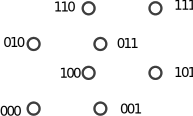
\includegraphics[width=2.111in, height=1.285in]{figures/hypercube}
    \caption{Hypercube topology}
    \label{fig:ch-ned-lang:hypercube-topology}
  \end{center}
\end{figure}


The hypercube topology\index{topology!hypercube} template is the
following (it can be placed into a separate file, e.g \ttt{Hypercube.ned}):

\begin{Verbatim}[commandchars=\\\{\}]
\tbf{simple} Node \{
    \tbf{gates}:
        \tbf{output} out[];
        \tbf{input} in[];
\}

\tbf{module} Hypercube \{
    \tbf{parameters}:
        int dim;
        string nodetype;
    \tbf{submodules}:
        node[2{\textasciicircum}dim]: <nodetype> \tbf{like} Node \{
        \tbf{gates}:
            out[dim];
            in[dim];
        \}
    \tbf{connections}:
        \tbf{for} i=0..2^dim-1, j=0..dim-1 \{
            node[i].out[j] --> node[i # 2^j].in[j]; // # is bitwise XOR
        \}
\}
\end{Verbatim}

When you create an actual hypercube, you substitute the name
of an existing module type (e.g. \ttt{"Hypercube\_PE"}) for the nodetype
parameter. The module type implements the algorithm the user
wants to simulate and it must have the same gates that the Node
type has. The topology template code can be used through importing
the file:

\begin{Verbatim}[commandchars=\\\{\}]
\tbf{simple} Hypercube_PE \{
    \tbf{gates}:
         \tbf{output} out[];
         \tbf{input} in[];
\}

\tbf{network} HypercubeX extends Hypercube \{
    \tbf{parameters}:
        dim = 4;
        nodetype = "Hypercube_PE";
\}
\end{Verbatim}

If you put the nodetype parameter to the ini file, you can use the
same simulation model to test e.g. several routing algorithms in a
hypercube, each algorithm implemented with a different
simple module type -- you just have to supply
different values to nodetype, such as \ttt{"WormholeRoutingNode"},
\ttt{"DeflectionRoutingNode"}, etc.



\section{Inheritance}
\label{sec:ch-ned-lang:inheritance}

Single inheritance is supported between modules, ie. you can further
specialize the above module:

XXX simple module inheritance

XXX compound module inheritance




\section{Interfaces, and submodule/channel type as parameter}
\label{sec:ch-ned-lang:like}

Sometimes it is convenient to make the name of a submodule type a parameter,
so that one can easily `plug in' any module there.

For example, assume the purpose of your simulation study is
to compare different routing algorithms. Suppose you programmed
the needed routing algorithms as simple modules: \ttt{DistVecRoutingNode},
\ttt{AntNetRouting1Node}, \ttt{AntNetRouting2Node}, etc.
You have also created the network topology as a compound module
called \ttt{RoutingTestNetwork}, which will serve as a testbed for your routing
algorithms. Currently, \ttt{RoutingTestNetwork} has \ttt{DistVecRoutingNode}
hardcoded (all submodules are of this type), but you want
to be able to switch to other routing algorithms easily.

NED gives you the possibility to add a string-valued parameter,
say \ttt{routingNodeType} to the \ttt{RoutingTestNetwork} compound module.
Then you can tell NED that types of the submodules inside \ttt{RoutingTestNetwork}
are not of any fixed module type, but contained in the \ttt{routingNodeType}
parameter. That is all -- now you are free to assign any of
the \ttt{"DistVecRoutingNode"}, \ttt{"AntNetRouting1Node"} or
\ttt{"AntNetRouting2Node"} string constants to this parameter
(you can do that in NED, in the config file (\ttt{omnetpp.ini}),
or even enter it interactively),
and your network will use the routing algorithm you chose.

If you specify a wrong value, say \ttt{"FooBarRoutingNode"}
when you have no \ttt{FooBarRoutingNode} module implemented,
you'll get a runtime error at the beginning of the simulation:
\textit{module type definition not found}.

Inside the \ttt{RoutingTestNetwork} module you assign parameter values
and connect the gates of the routing modules. To provide some degree
of type safety, NED wants to make sure you didn't misspell
parameter or gate names and you used them correctly.
To be able to do such checks, NED requires some help from you:
you have to name an existing module type (say \ttt{RoutingNode})
and promise NED that all modules you're going to specify
in the \ttt{routingNodeType} parameter will have (at least) the same
parameters and gates as the \ttt{RoutingNode} module.
  \footnote{If you like, the above solution somewhat similar to polymorphism
  in object-oriented languages -- \ttt{RoutingNode} is like a
  ``base class'', \ttt{DistVecRoutingNode} and \ttt{AntNetRouting1Node}
  are like ``derived classes'', and the \ttt{routingNodeType} parameter
  is like a ``pointer to a base class'' which may be downcast to specific
  types.}

All the above is achieved via the \fpar[ned!keywords!like]{like} keyword.
The syntax is the following:

\begin{Verbatim}[commandchars=\\\{\}]
\tbf{module} RoutingTestNetwork \{
    \tbf{parameters}:
        \tbf{string} routingNodeType; // should hold the name
                                      // of an existing module type
    \tbf{gates}: //...
    \tbf{submodules}:
        node1: <routingNodeType> \tbf{like} IRoutingNode;
        node2: <routingNodeType> \tbf{like} IRoutingNode;
        //...
    \tbf{connections allowunconnected}:
        node1.out0 --> node2.in0;
        //...
\}
\end{Verbatim}

The \ttt{RoutingNode} module type does not need to be implemented in
C++, because no instance of it is created; it is merely used
to check the correctness of the NED file.

On the other hand, the actual module types that will be substituted
(e.g. \ttt{DistVecRoutingNode}, \ttt{AntNetRouting1Node},etc.)
do not need to be declared in the NED files.

The \fpar[ned!keywords!like]{like} phrase lets you create families
of modules that serve similar purposes and implement the same interface
(they have the same gates and parameters)
and to use them interchangeably in NED files.



\section{Packages}

To address increasingly common name collisions in NED files,
{\opp} 4.0 introduces a package feature for NED. The solution
is roughly modelled after Java's packages, with minor enhancements.

It is also recommended practice to have one module per file,
and the file name to be the same as the module name (plus \ttt{.ned}).

\subsection{Packages, imports}

A NED file may contain a package declaration:

\begin{Verbatim}[commandchars=\\\{\}]
\tbf{package} inet.protocols.transport.tcp;
\end{Verbatim}

If there is no package declaration, the file is said to be in the
\textit{default package}.

Names from other NED files can be referred to either by fully qualified
name (\ttt{"inet.protocols.network.ip.RoutingTable"}), or by short name
(\ttt{"RoutingTable"}) if the name is visible.

Visible names are:
\begin{itemize}
  \item anything from the same package;
  \item imported names.
\end{itemize}

Import directives also have a similar syntax to Java, but they
are more flexible with wildcards. All of the following are legal:

\begin{Verbatim}[commandchars=\\\{\}]
\tbf{import} inet.protocols.network.ip.RoutingTable;
\tbf{import} inet.protocols.network.ip.*;
\tbf{import} inet.protocols.network.ip.Ro*Ta*;
\tbf{import} inet.protocols.*.ip.*;
\tbf{import} inet.**.RoutingTable;
\end{Verbatim}

One asterisk "*" stands for "any character sequence not containing
period"; two asterisks mean "any character sequence which may
contain period". No other wildcards are recognized.

An import not containing wildcard MUST match an existing NED type.
However, it is legal for an import that does contain wildcards
not to match any NED type (although that might generate a warning.)

Inner types may not be referred to outside their enclosing types.


\subsection{Directory Structure, package.ned}

Like in Java, the directory of a NED file MUST match the package declaration.
However, it is possible to omit directories at the top which don't
contain any NED files (like the "/org/projectname/" directories in Java).

There is a notion of "NED source folders". If a NED Source Folder is
named "src", then a NED file containing the package declaration
"inet.protocols.transport.tcp" must be in the following folder:

\begin{Verbatim}[commandchars=\\\{\}]
src/inet/protocols/transport/tcp/
\end{Verbatim}

If the "inet" and "protocols" directories don't contain any NED files,
they can be omitted:

\begin{Verbatim}[commandchars=\\\{\}]
src/transport/tcp
\end{Verbatim}

and the "src" directory must contain a "package.ned" file which declares
what package it corresponds to:

\begin{Verbatim}[commandchars=\\\{\}]
// file src/package.ned:
package inet.protocols;
\end{Verbatim}

All NED files under the "src" directory tree must have package
declarations consistent with that.

"package.ned" files are allowed in other folders as well (as long as
their package declarations are consistent with the NED source
directory's "package.ned"), and any file-level comment in them
will be treated as the package's documentation (similar to Java's
package.html).


\subsection{Name lookups}

\subsubsection{Base types and submodules}

Fully qualified names and simple names are accepted. Simple names
are looked up among the inner types of the enclosing type (compound
module), then using imports, then in the same package.


\subsubsection{Parametric module types ("like" submodules)}

Lookup of the actual module type for "like" submodules differs for normal
lookups. This lookup ignores the imports in the file altogether.
Instead, it collects all modules that support the given interface
and match the given type name string (i.e. end in the same simple name,
or have the same fully qualified name). The result must be exactly
one module type.

The algorithm for parametric channel types works in the same way.


\subsubsection{Network name in the ini file}

Simple (unqualified) names are tried with the same package as the
ini file is in (provided it's in a NED directory).

\subsection{The NEDPATH environment variable}

A simulation may need NED files from several "NED source folders".
When a simulation is launched as a separate application, it will expect
to receive the list of NED source folders to scan in the NEDPATH
environment variable (similar to Java's CLASSPATH). NEDPATH should
contain the source folder names separated by a semicolon (";").
On Unix-like systems, colon (":") will also be accepted as separator.

In the future, zip files may become supported in NEDPATH as well;
then the root folder of the zip file will be treated as a NED source
folder.


%%FIXME into other doc
\subsection{{\opp} Projects in Eclipse}

{\opp} projects within Eclipse are marked with the "{\opp} Nature",
that is, those projects marked with that nature will be recognized as
{\opp} projects.

NED source folders can only be located within {\opp} projects. (That is,
NED files within non-{\opp} projects will be always ignored.)

Which folders in a project are NED source folders is determined by
the ".nedfolders" file in the project root directory. This is a plain
text file, which contains directory names (as relative to the
project root directory), one per line. If the ".nedfolders" file is
missing, then the project root directory will be treated as the (only)
NED source folder.


%%FIXME into other doc
\subsection{Cross-Project Dependencies}

{\opp} projects in Eclipse may refer to NED files in other projects.
This feature is supported by making use of the Eclipse Platform's
support for project dependencies. (In the Eclipse Platform, for any
project one can define the list other projects it depends on.)

In one project, one may only refer to NED files in the same project
or dependent projects.




\section{XML as alternative representation of NED}

To increase interoperability, NED files (and also message definition files)
have an XML representation. Any NED file can be converted to XML, and
any XML file which corresponds to the NED DTD can be converted to NED.
  \footnote{DTD stands for Document Type Descriptor, and it defines
  a "grammar" for XML files. More info can be found on the W3C web site,
  www.w3.org.}

XML is well suited for machine processing. For example, stylesheet
transformations (XSLT) can be used to extract information from NED files,
or the other way round, create NED files from external info present in
XML form. One practical application of XML is the \fprog{opp\_neddoc}
documentation generation tool which is described in Chapter \ref{cha:neddoc}.

The \fprog{nedtool} program (which also translates NED to C++ code)
can be used to convert between NED and XML.

Converting a NED file to XML:

\begin{verbatim}
nedtool -x wireless.ned
\end{verbatim}

It generates \ttt{wireless\_n.xml}.
Several switches control the exact content and details
of the resulting XML as well as the amount of checks
made on the input.

Converting the XML representation back to NED:

\begin{verbatim}
nedtool -n wireless.xml
\end{verbatim}

The result is \ttt{wireless\_n.ned}.

Using nedtool as NED compiler to generate C++ code:

\begin{verbatim}
nedtool wireless.ned
\end{verbatim}

The resulting code is more compact than the
one created by \fprog{nedtool}'s predecessor \fprog{nedc}.
As a result, \fprog{nedtool}-created \ttt{\_n.cc}
C++ files compile much faster.

You can generate C++ code from the XML format as well:

\begin{verbatim}
nedtool wireless.xml
\end{verbatim}



\section{Large networks}

There are situations when using hand-written NED files to describe
network topology is inconvenient, for example when
the topology information comes from
an external source\index{topology!external source} like
a network management program.

In such case, you have two possibilities:

\begin{enumerate}
  \item{generating NED files from data files}
  \item{building the network from C++ code}
\end{enumerate}

The two solutions have different advantages and disadvantages.
The first is more useful in the model development phase, while
the second one is better for writing larger scale, more productized
simulation programs. In the next sections we examine both methods.



\subsection{Generating NED files}


Text processing programs like \fprog{awk} or \fprog{perl} are
excellent tools to read in textual data files and generate NED files
from them\index{ned!file generation}.  Perl also has extensions to
access SQL databases, so it can also be used if the network topology
is stored in a database.

The advantage is that the necessary \fprog{awk} or \fprog{perl}
program can be written in a relatively short time, and it is
inexpensive to maintain afterwards: if the structure of the data files
change, the NED-creating program can be easily modified. The
resulting NED files can either be translated by \fprog{nedtool}
into C++ and compiled in, or loaded dynamically.


\subsection{Building the network from C++ code}

Another alternative is to write C++ code which becomes part of the
simulation executable. The code would read the topology data from data
files or a database, and build the network directly, using
dynamic module creation (to be described later, in section
\ref{ch:simple-modules:dynamic-module-creation}).
The code which you need to write would be similar to the \ttt{*\_n.cc}
files output by \fprog{nedtool}.

Since writing such code is more complex than letting perl generate
NED files, this method is recommended when the simulation program
has to be somewhat more productized, for example when {\opp}
and the simulation model is embedded into a larger program, e.g.
a network design tool.


\section{Extending NED with new functions}
\index{ned!functions}
\label{sec:ch-ned-lang:defining-functions}

To use user-defined functions\index{functions!user-defined}, one has
to code the function in C++.  The C++ function must take 0, 1, 2, 3, or 4
arguments of type double and return a double. The function must be
registered in one of the C++ files with the \fmac{Define\_Function()}
macro.

An example function (the following code must appear in one of the C++
sources):


\begin{verbatim}
#include <omnetpp.h>

double average(double a, double b)
{
  return (a+b)/2;
}

Define_Function(average, 2);
\end{verbatim}

The number 2 means that the \fname{average()} function has 2
arguments. After this, the \fname{average()} function can be used in
NED files:

\begin{Verbatim}[commandchars=\\\{\}]
\tbf{module} Compound \{
    \tbf{parameters}:
        double a;
        double b;
    \tbf{submodules}:
        proc: Processor \{
            avg = average(a,b);
        \}
\}
\end{Verbatim}


If your function takes parameters that are \ttt{int} or \ttt{long} or
some other type which is not \ttt{double}, you can create wrapper function
that takes all doubles and does the conversion. In this case you have
to register the wrapper function with the \fname{Define\_Function2()} macro
which allows a function to be registered with a name different from the
name of the function that implements it. You can do the same
if the return value differs from \ttt{double}.

FIXME the new way...

\begin{verbatim}
#include <omnetpp.h>

long factorial(int k)
{
  ...
}

static double _wrap_factorial(double k)
{
  return factorial((int)k);
}

Define_Function2(factorial, _wrap_factorial, 1);
\end{verbatim}

%%% Local Variables:
%%% mode: latex
%%% TeX-master: "usman"
%%% End:



